\documentclass[12pt,a4paper,oneside]{article}
\usepackage[colorlinks=true, unicode]{hyperref}
\usepackage[utf8]{inputenc}
\usepackage[czech]{babel}
\usepackage{graphicx}
\usepackage{pdfpages}
\textwidth 16cm \textheight 25cm
\topmargin -1.3cm 
\oddsidemargin 0cm
\usepackage{footnote}
\pagestyle{empty}
\begin{document}
\title{Mikroprocesorový modul PIC18F4550v01A}
\author{Jakub Kákona, kaklik@mlab.cz}
\maketitle

\thispagestyle{empty}
\begin{abstract}
Poskytuje možnost připojení mikroprocesoru PIC18F4550 do vývojových aplikací.
\end{abstract}

\begin{figure} [htbp]
\begin{center}
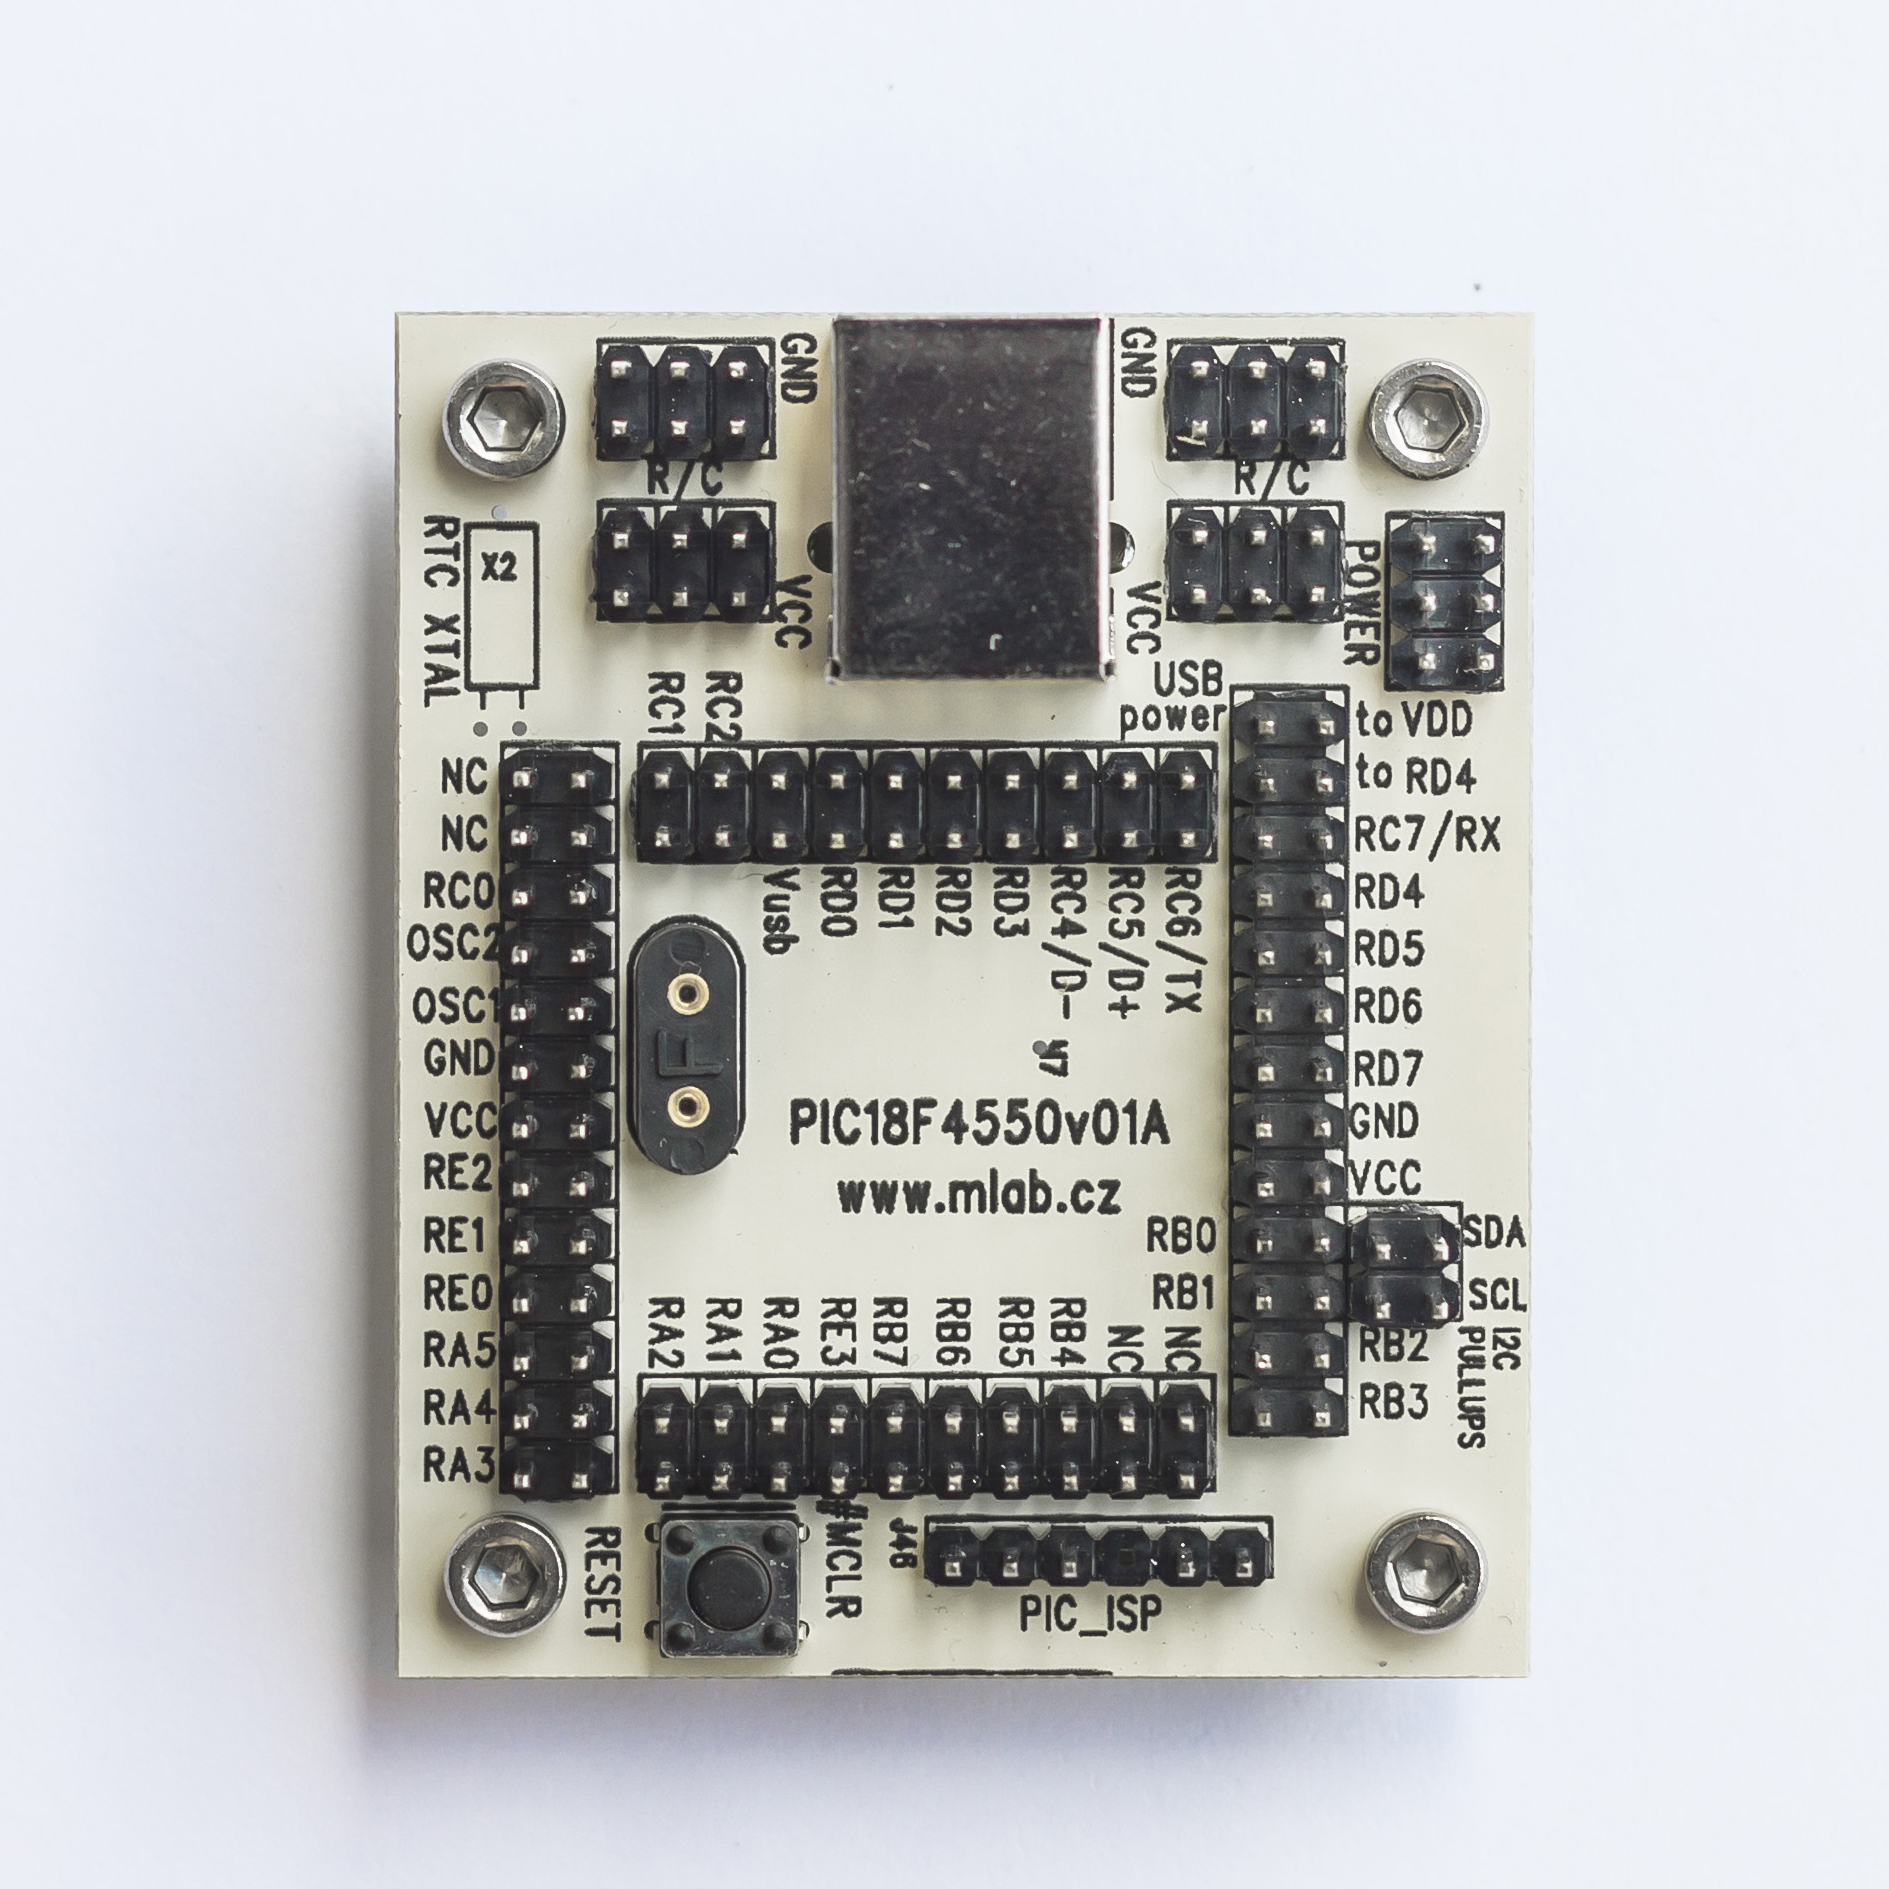
\includegraphics [width=100mm] {./img/PIC18F4550v01A_Top_Big.jpg} 
\end{center}
\end{figure}

\begin{figure} [b]

\includegraphics [width=25mm] {./img/PIC18F4550v01A_QRcode.png} 
\end{figure}

\newpage
\tableofcontents

\section{Technické parametry}
\begin{table}[htbp]
\begin{center}
\begin{tabular}{|c|c|p{4.7cm}|}
\hline
Parametr & Hodnota & Poznámka \\
\hline
Napájecí napětí POWER  & max 5V & \\ 
\hline
Digitální úrovně & CMOS &  Odpovídají napájecímu napětí. \\ 
\hline
\end{tabular}
\end{center}
\end{table}

\section{Popis konstrukce}

\subsection{Zapojení}
Modul obsahuje všechny potřebné podpůrné obvody pro provozování mikrokontroleru PIC18F4550. Do zapojení je možné připojit několik typů krystalových oscilátorů, je však potřeba pak přizpůsobit hodnotu rezonančních kondenzátorů. Doporučené hodnoty těchto kapacit lze najít v datasheetu k mikrokontroleru.  

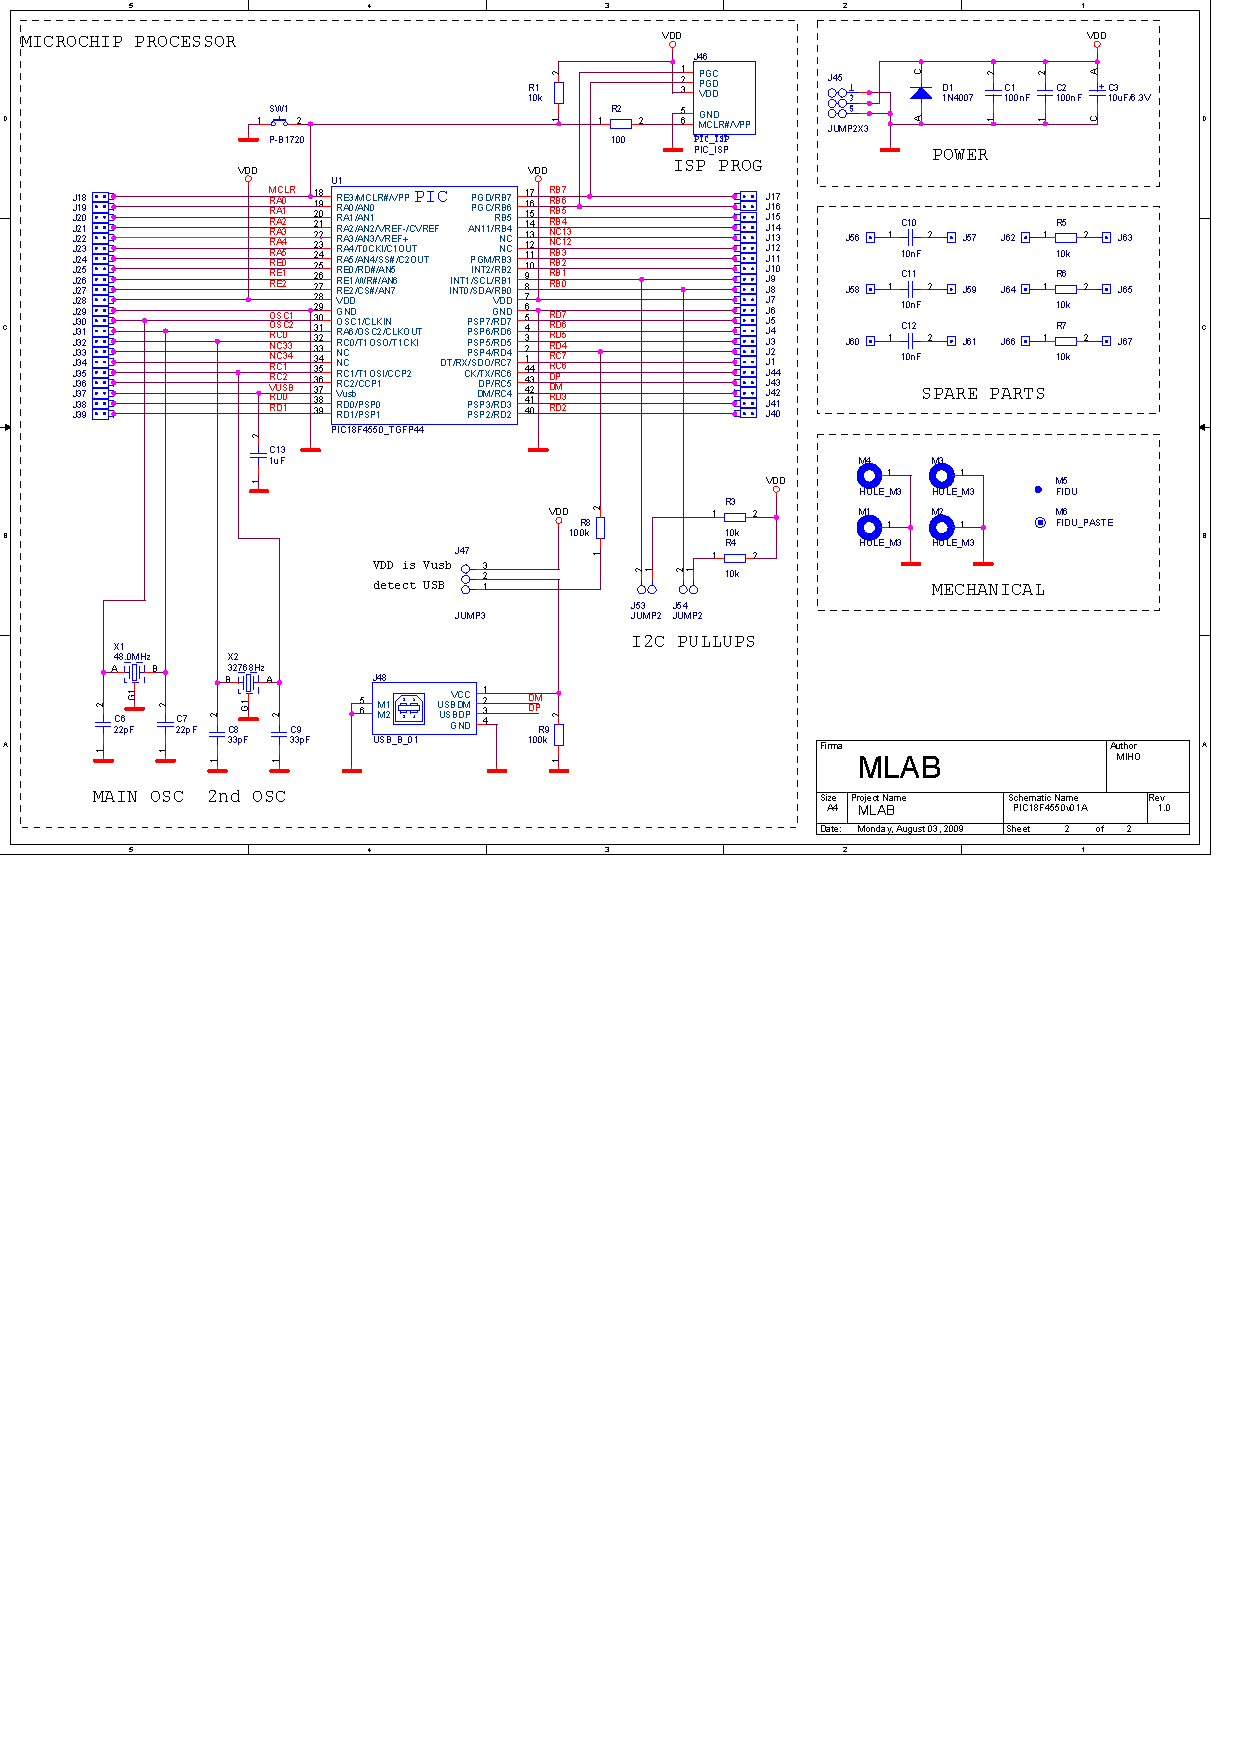
\includepdf[pages={1},landscape=false]{../../SCH/PIC18F4550V01A.pdf}

V zapojení modulu je obsažen lineární stabilizátor určený pro vytvoření napájecího napětí interní logiky USB.

\subsection{Mechanická konstrukce}

Modul klasicky předpokládá uchycení na čtyřech šroubech, z důvodu lepšího EMC odstínění je vhodné zabezpečit aby všechny šrouby byly vodivě spojeny s podložkou.  Předpokládá se, že USB-B konektor bude při použití modulu směřovat na okraj MLAB desky. 

\section{Výroba a testování}

Plošný spoj je navržen jak pro ruční pájení, tak i pro osazování pomocí pasty.  Modul se testuje optickou kontrolou spojů a následným připojením na laboratorní zdroj s omezením proudu.

\newpage

\begin{figure} [h!tbp]
  \centering
  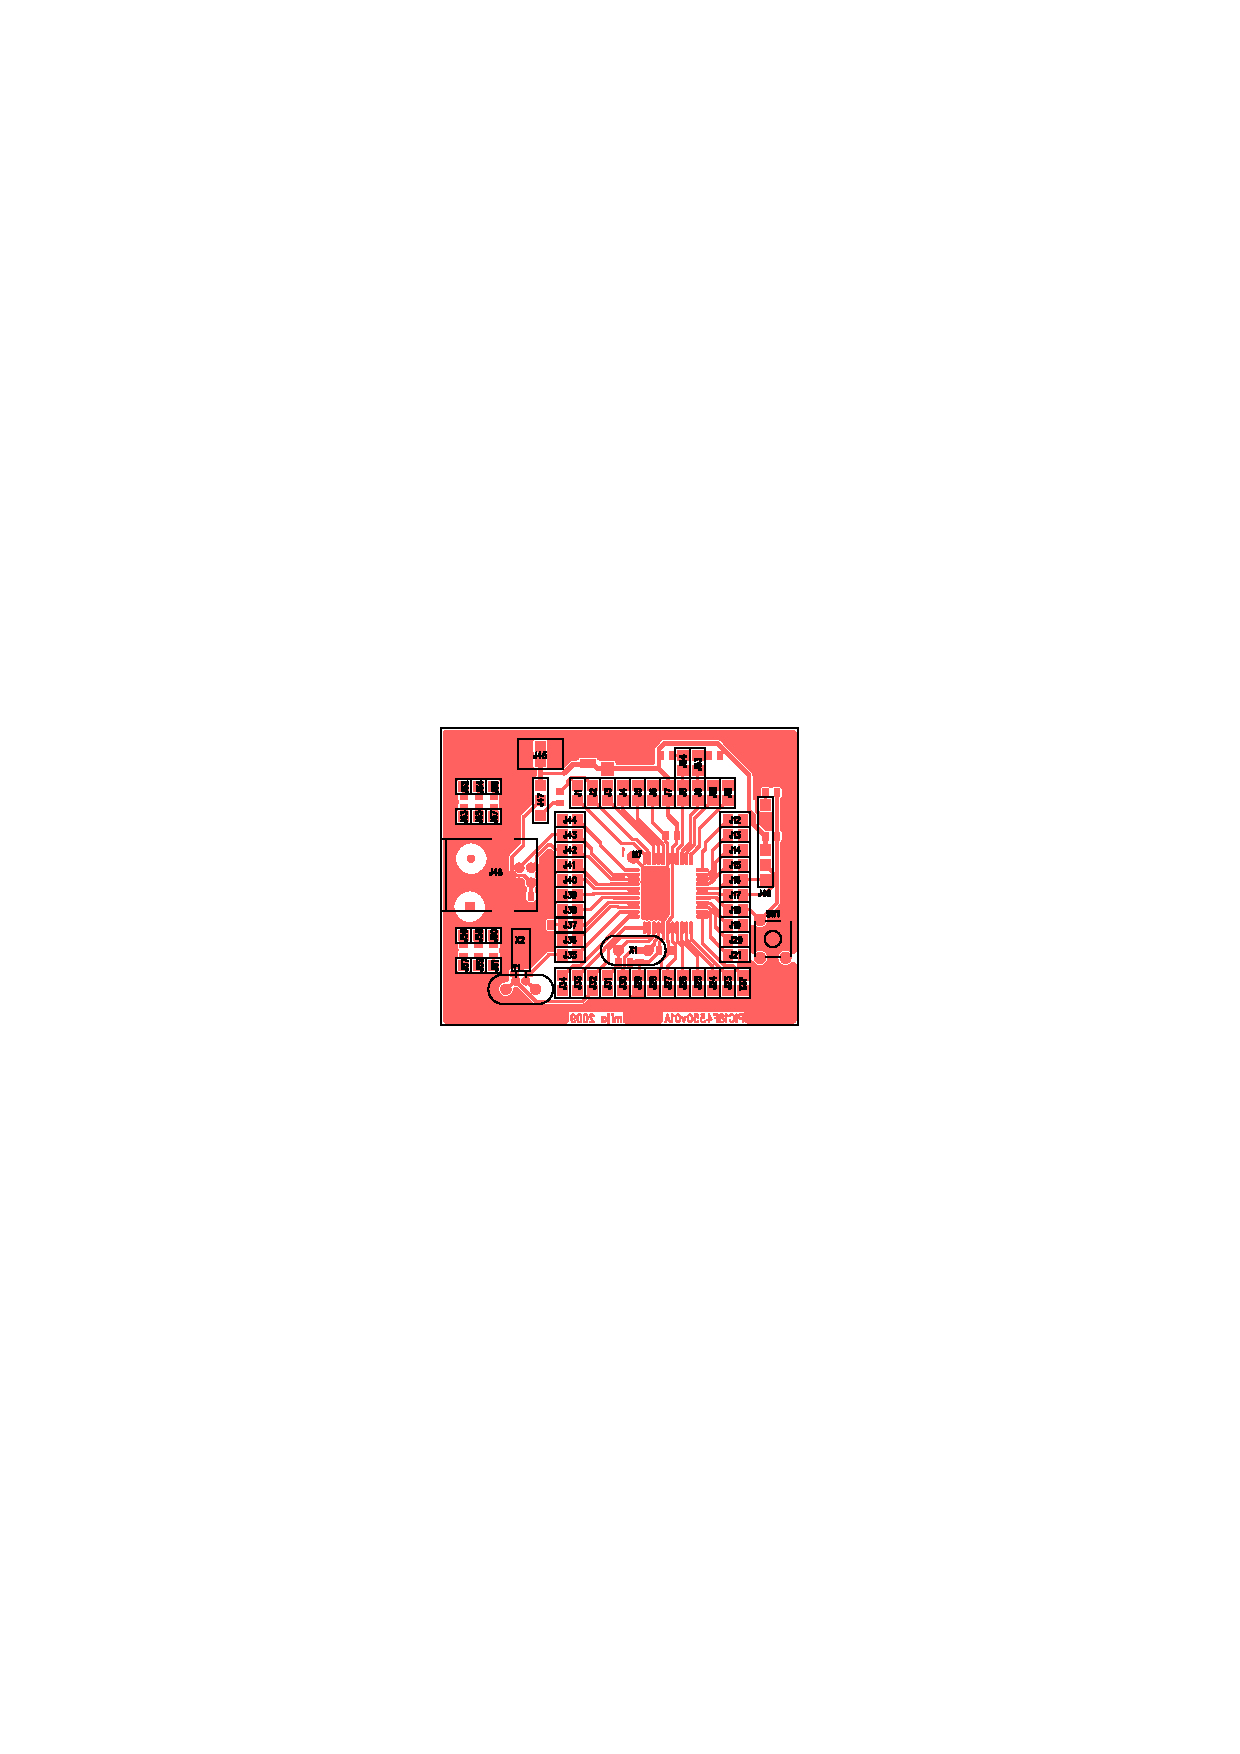
\includegraphics[trim = 7.0cm 12.0cm 7.0cm 12.0cm, clip, width=12cm]{../../CAM_DOC/O1.pdf}
  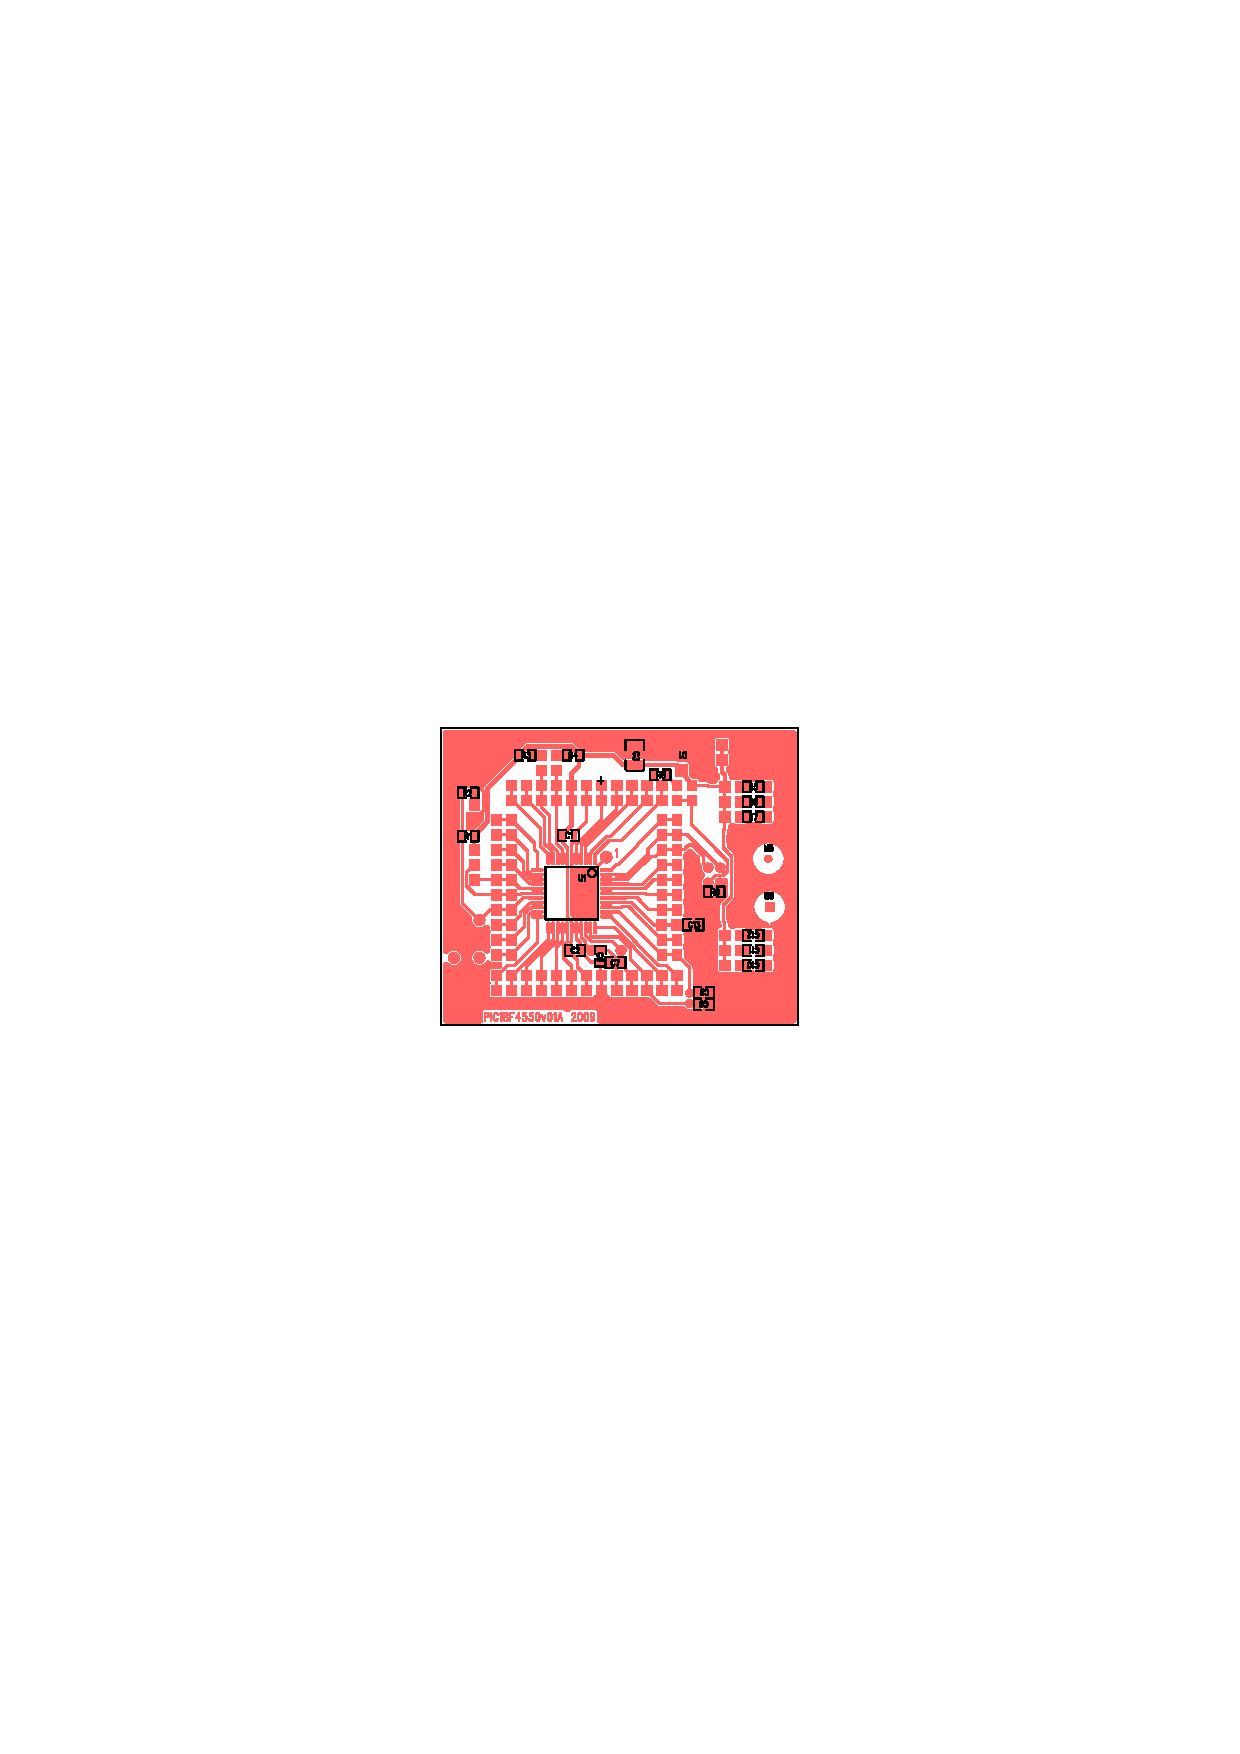
\includegraphics[trim = 7.0cm 12.0cm 7.0cm 12.0cm, clip, width=12cm]{../../CAM_DOC/O2.pdf}
  \caption{Osazovací plán horní a spodní strany plošného spoje}
  \label{fig:osazovaci_plan}
\end{figure}

\begin{savenotes}
\begin{table}[h!]
\begin{center}
\begin{tabular}{ |c|c|c|c| }
\hline 
Počet & Označení & Typ  & Pouzdro  \\ 
\hline 
2	&	C1,C2	&	100nF	&	0805	\\
1	&	C3	&	10uF/6.3V	&	ELYT-B	\\
2	&	C6,C7	&	15pF	&	0805	\\
2	&	C8,C9	&	33pF	&	0805	\\
3	&	C10,C11,C12	&	10nF	&	0805	\\
1	&	C13	&	1uF	&	0805	\\
1	&	D1	&	M4	&	SMA	\\
46	&	J1,J2,J3,J4,J5,J6,J7,J8,	&	JUMP2	&		\\
	&	J9,J10,J11,J12,J13,J14,	&		&		\\
	&	J15,J16,J17,J18,J19,J20,	&		&		\\
	&	J21,J22,J23,J24,J25,J26,	&		&		\\
	&	J27,J28,J29,J30,J31,J32,	&		&		\\
	&	J33,J34,J35,J36,J37,J38,	&		&		\\
	&	J39,J40,J41,J42,J43,J44,	&		&		\\
	&	J53,J54	&		&		\\
1	&	J45	&	JUMP2X3	&		\\
1	&	J46	&	PIC\_ISP	&		\\
1	&	J47	&	JUMP3	&		\\
1	&	J48	&	USB\_B\_01	&		\\
12	&	J56,J57,J58,J59,J60,J61, J62,J63,J64,J65,J66,J67	&	JUMP1	&		\\
6	&	R1,R3,R4,R5,R6,R7	&	10k	&	0805	\\
1	&	R2	&	100	&	0805	\\
2	&	R8,R9	&	100k	&	0805	\\
1	&	SW1	&	P-B1720	&		\\
1	&	U1	&	PIC18F4550	&	TQFP44	\\
1	&	X1	&	20.0MHz	&		\\
1	&	X2	&	32768Hz	&		\\
\hline 
\end{tabular}
\end{center}
\caption{Seznam součástek potřebných pro sestavení modulu.}
\label{seznam_soucastek}
\end{table}
\end{savenotes}

\newpage

\section{Programové vybavení}

Pro použití modulu je potřeba do mikrokontroleru nahrát firmware, který zkompilujeme v některém vývojovém nástroji pro Microchip, jako je například CCS C, nebo MPLAB.

\begin{thebibliography}{99}

\end{thebibliography}
\end{document}